\section{Lastenheft}
  \subsection{Berechnung der Vertikalen Beschleunigung}
  \label{Vertikale Beschleunigung}
  Die Position des Rades während dem Überfahren der Bremsschwelle ist gegeben durch folgenden Zusammenhang:
  \begin{equation}
    x_r^n = h \cdot sin\left(\pi \cdot \frac{n \cdot \Delta t \cdot v}{l}\right)
  \end{equation}
  $l$ steht dabei für die Länge, und h für die Höhe der Bremsschwelle. $v$ für die Geschwindigkeit des Solar Butterflys beim Überfahren, $n$ für den Zeitschritt und $\Delta t$ für die Zeitinkrementierung pro Berechnungsschritt.\\

  Um die Beschleunigung des Solar Butterflys zu berechnen, wird in einem ersten Schritt dessen Position zum Zeitpunk $n$ $x_{SB}^n$ aus der vorangehenden Situation berechnet.
  \begin{equation}
    x_{SB}^n = x_{SB}^{(n-1)} + v^{(n-1)} \cdot \Delta t
  \end{equation}

  Als nächstes wird der Federweg $s^n$, sowie die Änderungsrate des Federwegs $v_s^n$ zum Zeitpunkt $n$ aus den Positionen des Rades $r_x^n$ und des Solar Butterflys $x_{SB}^n$ berechnet.
  \begin{equation}
    s^n = x_r^n - x_{SB}^n
  \end{equation}
  \begin{equation}
    v_s^n = \frac{s^n - s^{(n-1)}}{\Delta t}
  \end{equation}

  Die Beschleunigung des Solar Butterfly ergibt sich dann zu:\\
  \begin{equation}
    a_{SB}^n = \frac{k \cdot s^n + d \cdot v_s^n}{m}
  \end{equation}

  Wobei $k$ für die Federkonstante und $d$ für die Dämpfungskonstante stehen.
  Die aus der Beschleunigung des Solar Butterfly resultierende neue Geschwindigkeit, kann wie folgt berechnet werden.
  \begin{equation}
    v^n = v^{(n-1)} + a_{SB}^n \cdot \Delta t
  \end{equation}



\section{FEM}

\subsection{FEM Ergebnisse}
  \label{FEM Ergebnisse}

  \subsubsection{FEM-Ergebnis - Lastfall 1.1 Vertikale Beschleunigung}
  \begin{table}[H]
  \centering
  \begin{tabular}{lcccccc}
  Grösse	&	Einheit	&	x	&	y	&	z	&	Total	&	Berechnet	\\	\hline
  \multicolumn{5}{l}{\textbf{Lagerreaktionen}}									&		&		\\	\thickhline
  Deichsel	&	N	&	0	&	3177	&	0	&	3177	&	-1028 (y)	\\
  Chassis Links	&	N	&	0	&	35073	&	6705	&	35708	&	37300 (y)	\\
  Chassis Rechts	&	N	&	0	&	35073	&	-6705	&	35708	&	37300 (y)	\\	\hline	\\
  \multicolumn{5}{l}{\textbf{Chassis}}									&		&		\\	\thickhline
  Axialkraft	&	N	&		&		&		&	-50809	&	-47425	\\
  Querkraft	&	N	&		&		&		&	16968	&	18222	\footnotemark \\
  Biegemoment	&	kNmm	&		&		&		&	16961	&		\\	\hline	\\
  \multicolumn{5}{l}{\textbf{Dach}}									&		&		\\	\thickhline
  Axialkraft	&	N	&		&		&		&	1951	&	15808	\\
  Querkraft	&	N	&		&		&		&	93	&		\\
  Biegemoment	&	kNmm	&		&		&		&	38	&		\\	\hline	\\
  \multicolumn{5}{l}{\textbf{Träger A und B}}													\\	\thickhline
  Axialkraft	&	N	&		&		&		&	-10857	&		\\
  Querkraft	&	N	&		&		&		&	1290	&		\\
  Biegemoment	&	kNmm	&		&		&		&	326	&		\\	\hline	\\
  \multicolumn{5}{l}{\textbf{Kontaktreaktion: Chassis - Träger A und B}}									&		&		\\	\thickhline
  Axialkraft A	&	N	&	619	&	12961	&	276	&	12978	&		\\
  Biegemoment A	&	kNmm	&	4606	&	179	&	340	&	4622	&		\\
  Axialkraft B	&	N	&	2449	&	15846	&	707	&	16036	&		\\
  Biegemoment B	&	kNmm	&	5626	&	845	&	345	&	5695	&		\\	\hline	\\
  \multicolumn{5}{l}{\textbf{Kontaktreaktion: Chassis - Boden}}									&		&		\\	\thickhline
  Normalkraft (Zug)	&	N	&		&		&		&	883	&		\\
  Schubkraft (xz-Ebene)	&	N	&		&		&		&	9933	&		\\	\hline
  \end{tabular}
  \caption{Resultate der FEM-Simulation des Lastafalles der vertikalen Beschleunigung}
  \label{tab:FEM 1.1}
  \end{table}
  \footnotetext[2]{Unter der Annahme, dass nur das Chassis Querkräfte aufnimmt. Die Kraft von 19 kN ergibt sich aus der Halbierung der globalen Querkraft aus der Berechnung im Kapitel \ref{1.1 Vertikale Beschleunigung}.}

  \subsubsection{FEM-Ergebnis - Lastfall 1.3 Longitudinale Beschleunigung negativ}
  \begin{table}[H]
  \centering
  \begin{tabular}{lcccccc}
  Grösse	&	Einheit	&	x	&	y	&	z	&	Total	&	Berechnet	\\	\hline
  \multicolumn{5}{l}{\textbf{Lagerreaktionen}}									&		&		\\	\thickhline
  Deichsel	&	N	&	20551	&	3031	&	0	&	20773	&	20600 (x)	\\
  Chassis Links	&	N	&	0	&	-1515	&	-512	&	1600	&		\\
  Chassis Rechts	&	N	&	0	&	-1515	&	512	&	1600	&		\\	\hline	\\
  \multicolumn{5}{l}{\textbf{Chassis}}									&		&		\\	\thickhline
  Axialkraft	&	N	&		&		&		&	-6065	&		\\
  Querkraft	&	N	&		&		&		&	1308	&		\\
  Biegemoment	&	kNmm	&		&		&		&	2588	&		\\	\hline	\\
  \multicolumn{5}{l}{\textbf{Dach}}									&		&		\\	\thickhline
  Axialkraft	&	N	&		&		&		&	-379	&		\\
  Querkraft	&	N	&		&		&		&	4	&		\\
  Biegemoment	&	kNmm	&		&		&		&	1	&		\\	\hline	\\
  \multicolumn{5}{l}{\textbf{Träger A und B}}													\\	\thickhline
  Axialkraft	&	N	&		&		&		&	1551	&		\\
  Querkraft	&	N	&		&		&		&	55	&		\\
  Biegemoment	&	kNmm	&		&		&		&	17	&		\\	\hline	\\
  \multicolumn{5}{l}{\textbf{Kontaktreaktion: Chassis - Träger A und B}}									&		&		\\	\thickhline
  Axialkraft A	&	N	&	56	&	2086	&	323	&	2111	&		\\
  Biegemoment A	&	kNmm	&	735	&	19	&	2	&	735	&		\\
  Axialkraft B	&	N	&	96	&	664	&	79	&	674	&		\\
  Biegemoment B	&	kNmm	&	234	&	33	&	14	&	237	&		\\	\hline	\\
  \multicolumn{5}{l}{\textbf{Kontaktreaktion: Chassis - Boden}}									&		&		\\	\thickhline
  Normalkraft (Zug)	&	N	&		&		&		&	288	&		\\
  Schubkraft (xz-Ebene)	&	N	&		&		&		&	1731	&		\\	\hline
  \end{tabular}
  \caption{Resultate der FEM-Simulation des Lastafalles der longitudinalen Beschleunigung}
  \label{tab:FEM 1.3}
  \end{table}



  \subsubsection{FEM-Ergebnis - Lastfall 1.4 laterale Beschleunigung}
  \begin{table}[H]
  \centering
  \begin{tabular}{lcccccc}
  Grösse	&	Einheit	&	x	&	y	&	z	&	Total	&	Berechnet	\\	\hline
  \multicolumn{5}{l}{\textbf{Lagerreaktionen}}									&		&		\\	\thickhline
  Deichsel	&	N	&	0	&	0	&	1018	&	1018	&	-330 (z)	\\
  Chassis Links	&	N	&	0	&	-14911	&	11258	&	18684	&	11900 (z)	\\
  Chassis Rechts	&	N	&	0	&	14911	&	11211	&	18655	&	11900 (z)	\\	\hline	\\
  \multicolumn{5}{l}{\textbf{Chassis}}									&		&		\\	\thickhline
  Axialkraft	&	N	&		&		&		&	-31744	&	11711	\\
  Querkraft	&	N	&		&		&		&	7123	&	6100	\footnotemark \\
  Biegemoment	&	kNmm	&		&		&		&	6628	&		\\	\hline	\\
  \multicolumn{5}{l}{\textbf{Dach}}									&		&		\\	\thickhline
  Axialkraft	&	N	&		&		&		&	-1731	&	-732	\\
  Querkraft	&	N	&		&		&		&	14	&		\\
  Biegemoment	&	kNmm	&		&		&		&	9	&		\\	\hline	\\
  \multicolumn{5}{l}{\textbf{Träger A und B}}													\\	\thickhline
  Axialkraft	&	N	&		&		&		&	2654	&		\\
  Querkraft	&	N	&		&		&		&	1071	&	470	\\
  Biegemoment	&	kNmm	&		&		&		&	639	&	470	\\	\hline	\\
  \multicolumn{5}{l}{\textbf{Kontaktreaktion: Chassis - Träger A und B}}									&		&		\\	\thickhline
  Axialkraft A	&	N	&	237	&	3527	&	1748	&	3935	&		\\
  Biegemoment A	&	kNmm	&	1919	&	71	&	101	&	1923	&		\\
  Axialkraft B	&	N	&	720	&	4180	&	1711	&	4565	&		\\
  Biegemoment B	&	kNmm	&	2092	&	246	&	94	&	2109	&		\\	\hline	\\
  \multicolumn{5}{l}{\textbf{Kontaktreaktion: Chassis - Boden}}									&		&		\\	\thickhline
  Normalkraft (Zug)	&	N	&		&		&		&	1942	&		\\
  Schubkraft (xz-Ebene)	&	N	&		&		&		&	10972	&		\\	\hline
  \end{tabular}
  \caption{Resultate der FEM-Simulation des Lastafalles der lateralen Beschleunigung}
  \label{tab:FEM 1.4}
  \end{table}
  \footnotetext[3]{Unter der Annahme, dass nur das Chassis Querkräfte aufnimmt. Die Kraft von 6.1 kN ergibt sich aus der Halbierung der globalen Querkraft aus der Berechnung im Kapitel \ref{1.4 Laterale Beschleunigung}.}


  \subsubsection{FEM-Ergebnis - Lastfall 1.5 Rotatorische Beschleunigung}
  \begin{table}[H]
  \centering
  \begin{tabular}{lcccccc}
  Grösse	&	Einheit	&	x	&	y	&	z	&	Total	&	Berechnet	\\	\hline
  \multicolumn{5}{l}{\textbf{Lagerreaktionen}}									&		&		\\	\thickhline
  Deichsel	&	N	&	0	&	0	&	795	&	795	&		\\
  Chassis Links	&	N	&	0	&	-22915	&	10864	&	25359	&	-27000 (y)	\footnotemark \\
  Chassis Rechts	&	N	&	0	&	22915	&	10795	&	25330	&	27000 (y)	\\	\hline	\\
  \multicolumn{5}{l}{\textbf{Chassis}}									&		&		\\	\thickhline
  Axialkraft	&	N	&		&		&		&	-44172	&		\\
  Querkraft	&	N	&		&		&		&	10927	&		\\
  Biegemoment	&	kNmm	&		&		&		&	10154	&		\\	\hline	\\
  \multicolumn{5}{l}{\textbf{Dach}}									&		&		\\	\thickhline
  Axialkraft	&	N	&		&		&		&	-2450	&		\\
  Querkraft	&	N	&		&		&		&	32	&		\\
  Biegemoment	&	kNmm	&		&		&		&	19	&		\\	\hline	\\
  \multicolumn{5}{l}{\textbf{Träger A und B}}													\\	\thickhline
  Axialkraft	&	N	&		&		&		&	-4066	&		\\
  Querkraft	&	N	&		&		&		&	1311	&		\\
  Biegemoment	&	kNmm	&		&		&		&	788	&		\\	\hline	\\
  \multicolumn{5}{l}{\textbf{Kontaktreaktion: Chassis - Träger A und B}}									&		&		\\	\thickhline
  Axialkraft A	&	N	&	372	&	5442	&	2372	&	5937	&		\\
  Biegemoment A	&	kNmm	&	2754	&	112	&	162	&	2761	&		\\
  Axialkraft B	&	N	&	1289	&	6335	&	2265	&	6840	&		\\
  Biegemoment B	&	kNmm	&	2983	&	444	&	156	&	3020	&		\\	\hline	\\
  \multicolumn{5}{l}{\textbf{Kontaktreaktion: Chassis - Boden}}									&		&		\\	\thickhline
  Normalkraft (Zug)	&	N	&		&		&		&	3118	&		\\
  Schubkraft (xz-Ebene)	&	N	&		&		&		&	10761	&		\\	\hline
  \end{tabular}
  \caption{Resultate der FEM-Simulation des Lastafalles der rotatorischen Beschleunigung}
  \label{tab:FEM 1.5}
  \end{table}
  \footnotetext[4]{Die Kräfte von  $\pm$ 27 kN ergeben sich aus der Halbierung der Kraft F aus der Berechnung im Kapitel \ref{1.5 Rotatorische Beschleunigung}.}


  \subsubsection{FEM-Ergebnis - Kontaktreaktion Träger A und B zu Chassis}
  \label{sec:FEMres Träger}
  \begin{table}[H]
  \centering
  \begin{tabular}{lcccccccccc}
  \thickhline
  	&	\multicolumn{4}{c}{Axialkraft [N]}							&	&	&	\multicolumn{4}{c}{Biegemoment [kNmm]}							\\
  Lastfall / Träger	&	x	&	y	&	z	&	total	&	&	&	x	&	y	&	z	&	total	\\	\hline
  1.1 A	&	56	&	2086	&	323	&	2111	&	&	&	735	&	19	&	2	&	735	\\
  1.1 B	&	96	&	664	&	79	&	674	&	&	&	234	&	33	&	14	&	237	\\
  1.2 A	&	56	&	2086	&	323	&	2111	&	&	&	735	&	19	&	2	&	735	\\
  1.2 B	&	96	&	664	&	79	&	674	&	&	&	234	&	33	&	14	&	237	\\
  1.4 A	&	237	&	3527	&	1748	&	3935	&	&	&	1919	&	71	&	101	&	1923	\\
  1.4 B	&	720	&	4180	&	1711	&	4565	&	&	&	2092	&	246	&	94	&	2109	\\
  1.5 A	&	372	&	5442	&	2372	&	5937	&	&	&	2754	&	112	&	162	&	2761	\\
  1.5 B	&	1289	&	6335	&	2265	&	6840	&	&	&	2983	&	444	&	156	&	3020	\\	\hline
  Max	&	1289	&	6335	&	2372	&	6840	&	&	&	2983	&	444	&	162	&	3020	\\	\thickhline
  \end{tabular}
  \caption{Maximale Axialkräfte und Biegemomente in den Trägern A und B in den unterschiedlichen Lastfällen}
  \label{tab:FEMres Träger Kont}
  \end{table}
  
  \newpage

\subsection{Deformationen}
\label{FEM Deformation}
\subsubsection{Deformation - Lastfall 1.1 Vertikale Beschleunigung}
\begin{figure}[H]
  \centering
  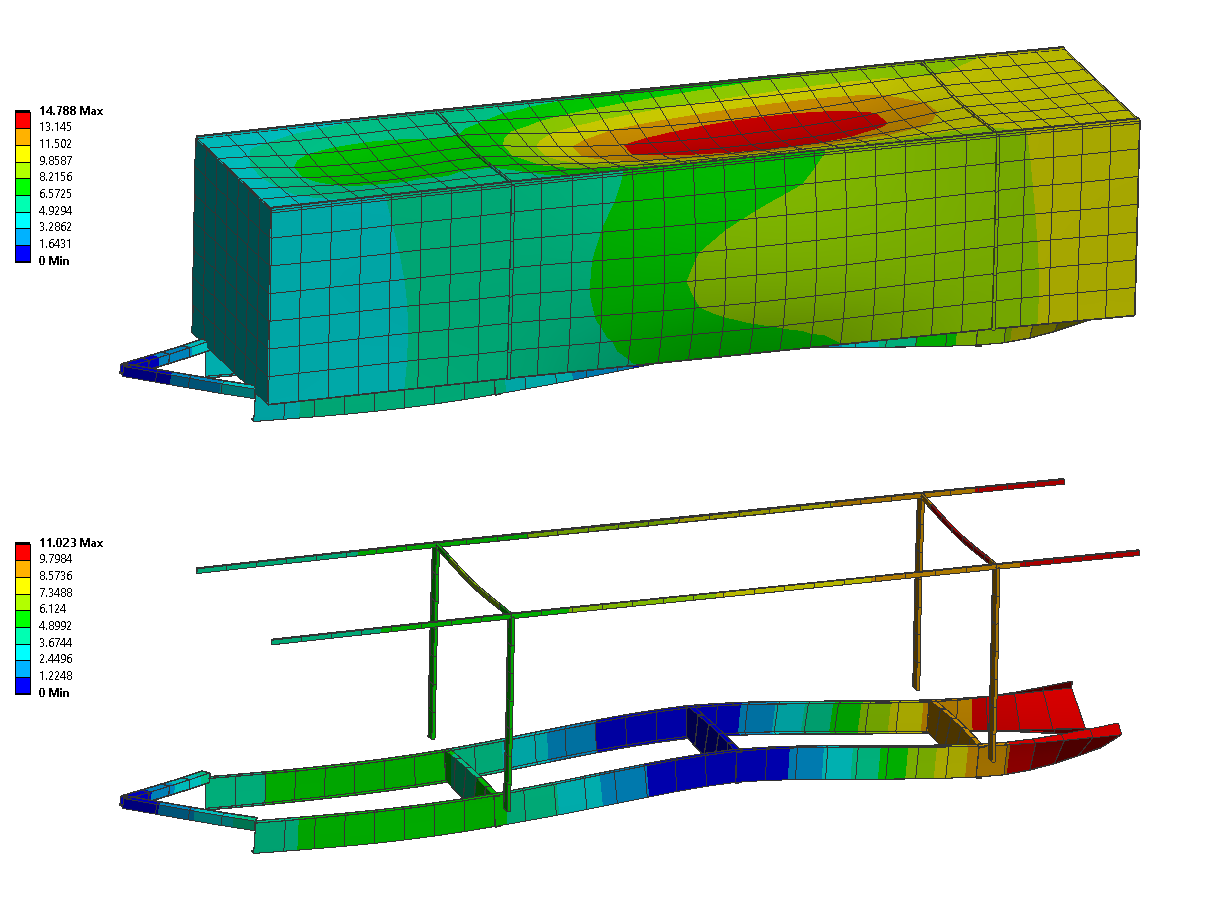
\includegraphics[width=1\linewidth]{04_figures/FEM 1.1.png}
  \caption{Deformation des Solar Butterflys im Lastfall der vertikalen Beschleunigung}
  \label{FEM 1.1}
\end{figure}

\subsubsection{Deformation - Lastfall 1.3 Longitudinale Beschleunigung}
\begin{figure}[H]
  \centering
  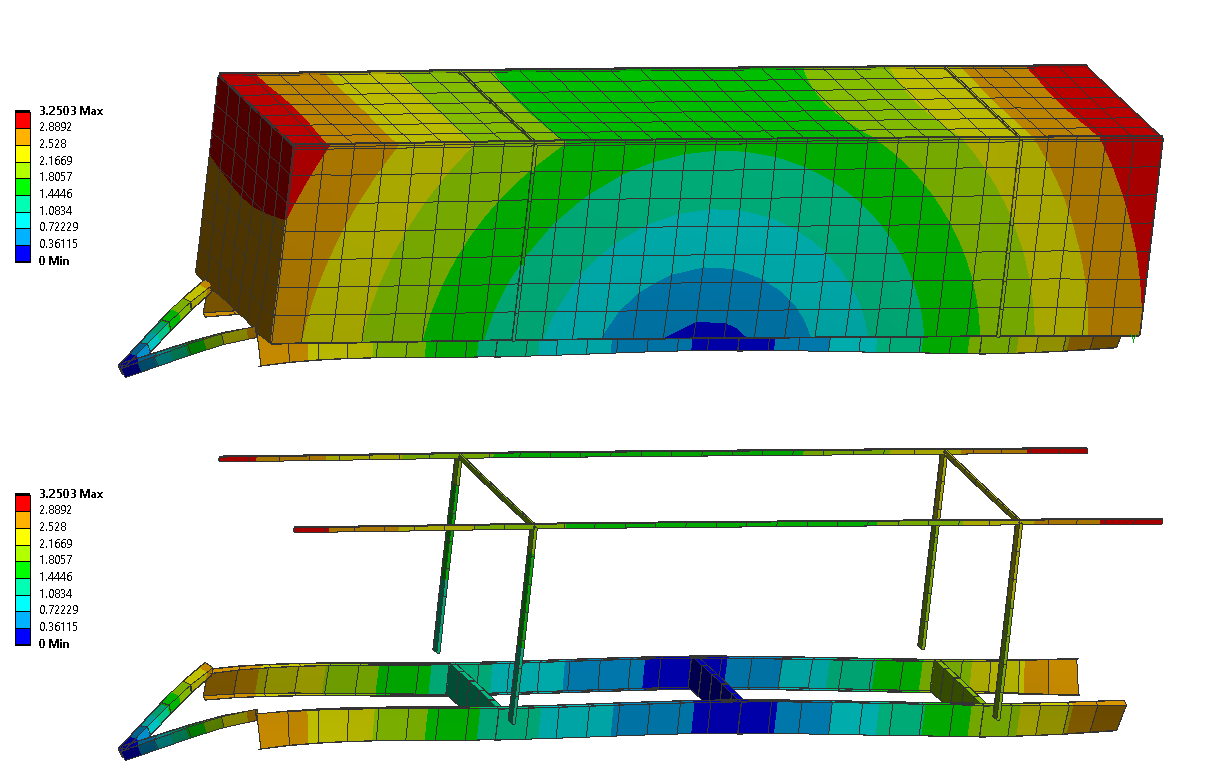
\includegraphics[width=1\linewidth]{04_figures/FEM 1.2.png}
  \caption{Deformation des Solar Butterflys im Lastfall der lateralen Beschleunigung}
  \label{FEM 1.3}
\end{figure}

\subsubsection{Deformation - Lastfall 1.4 Laterale Beschleunigung}
\begin{figure}[H]
  \centering
  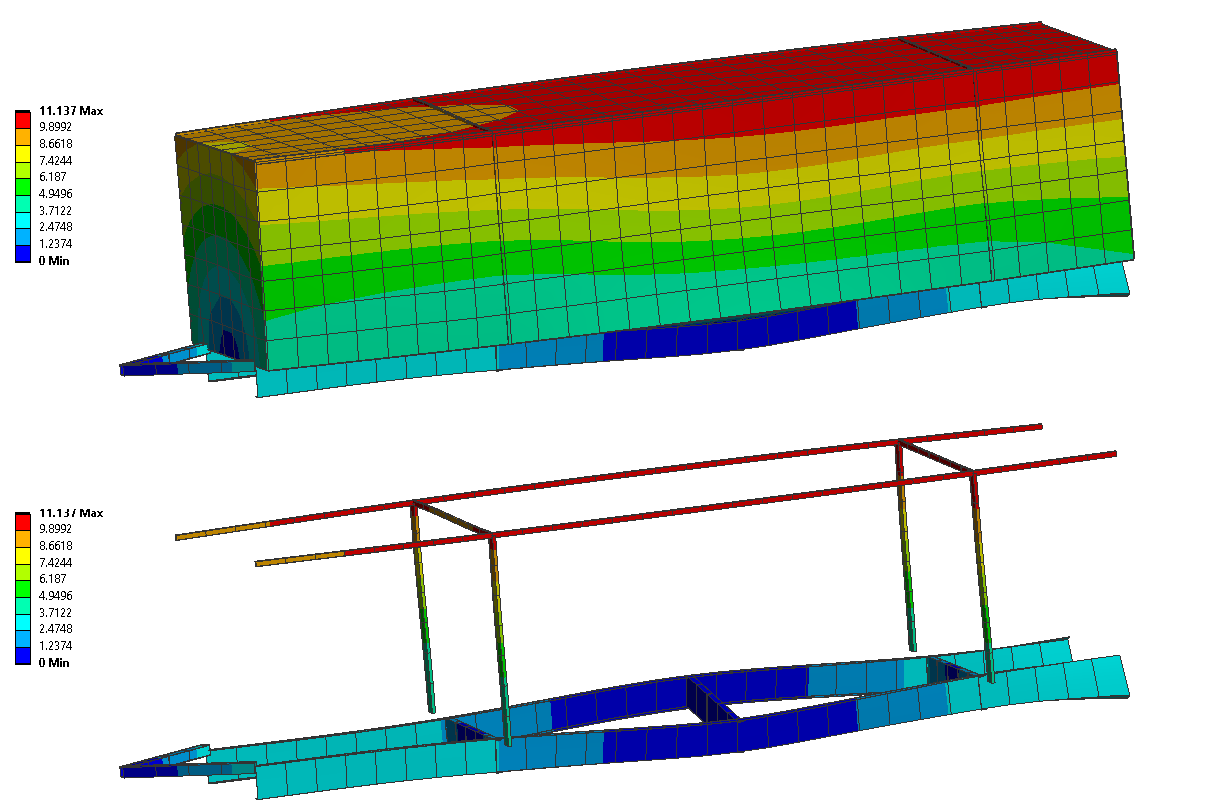
\includegraphics[width=1\linewidth]{04_figures/FEM 1.4.png}
  \caption{Deformation des Solar Butterflys im Lastfall der longitudinalen Beschleunigung}
  \label{FEM 1.4}
\end{figure}

\subsubsection{Deformation - Lastfall 1.5 Rotatorische Beschleunigung}
\begin{figure}[H]
  \centering
  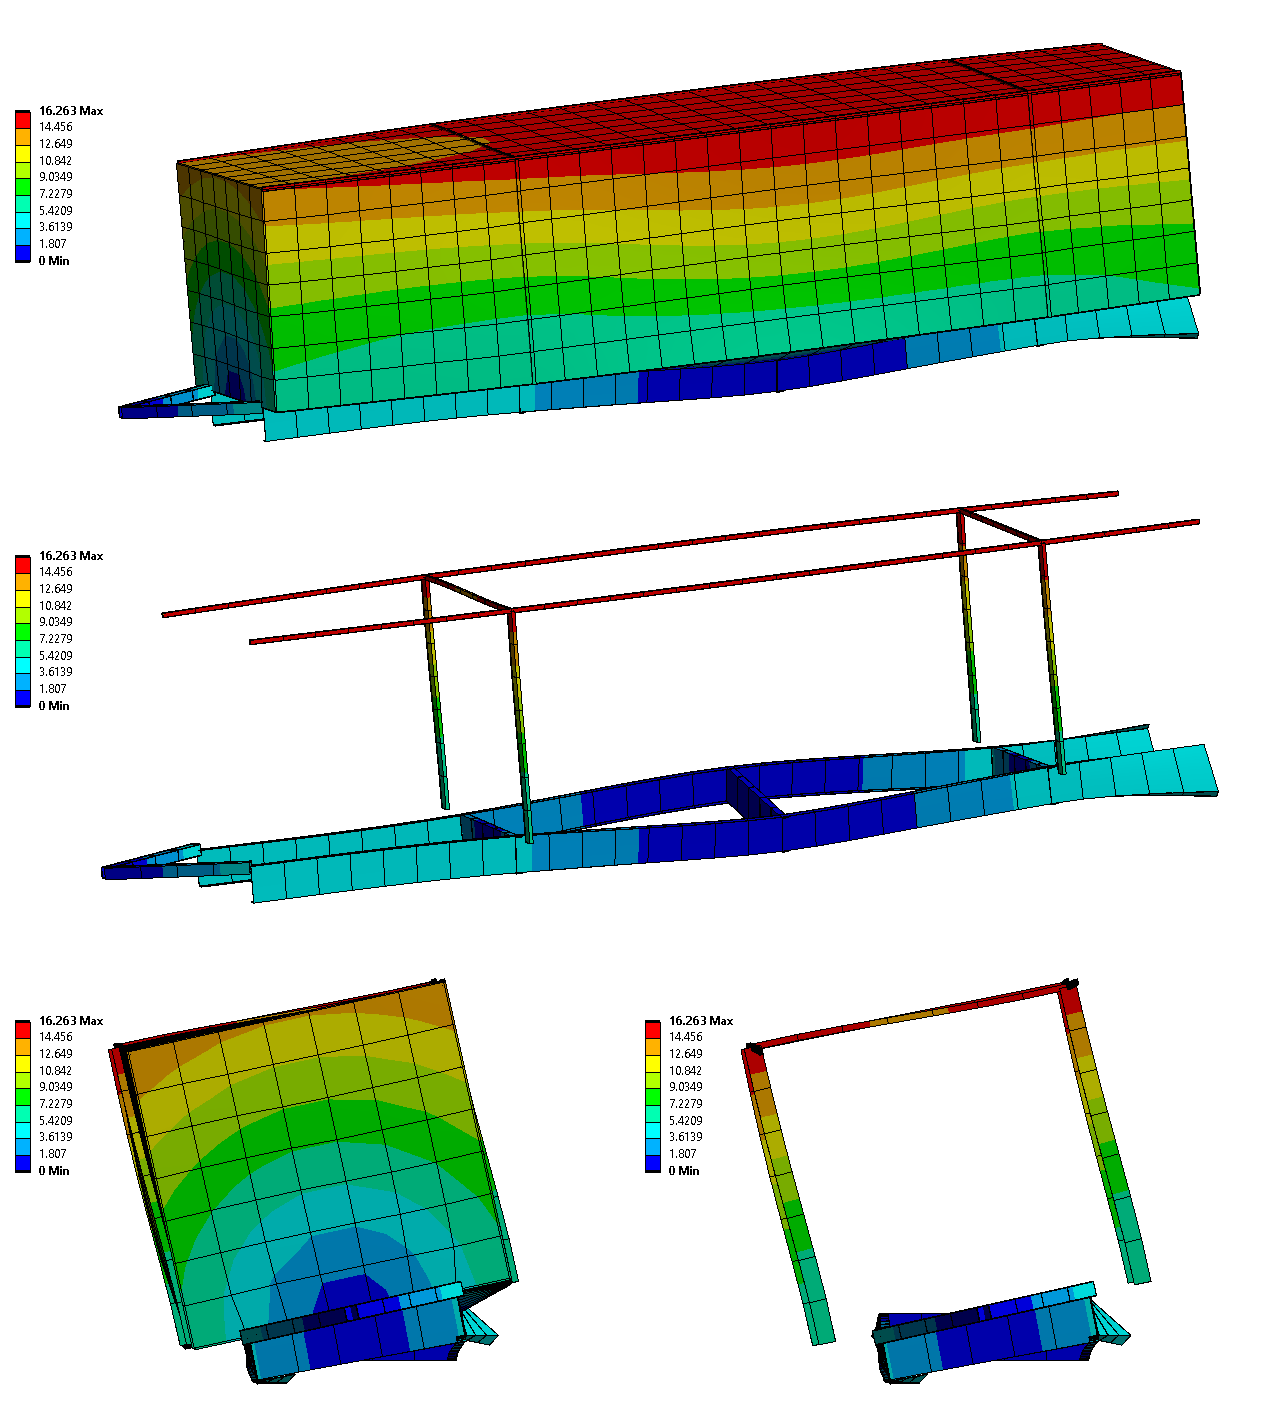
\includegraphics[width=1\linewidth]{04_figures/FEM 1.5.png}
  \caption{Deformation des Solar Butterflys im Lastfall der rotatorischen Beschleunigung}
  \label{FEM 1.5}
\end{figure}
\newpage
